\documentclass[10pt,twocolumn]{article}

\usepackage[T1]{fontenc}
\usepackage[utf8]{inputenc}
\usepackage{lmodern}
\usepackage[letterpaper,margin=0.75in,columnsep=0.25in]{geometry}
\usepackage{microtype}
\usepackage{amsmath,amssymb}
\usepackage{booktabs}
\usepackage{tabularx}
\usepackage{array}
\usepackage{enumitem}
\usepackage{xcolor}
\usepackage{tikz}
\usetikzlibrary{arrows.meta,fit,positioning,shapes.geometric}
\usepackage{pgfplots}
\usepackage{pgfplotstable}
\pgfplotsset{compat=1.18}
\usepackage[round,authoryear]{natbib}
\usepackage{doi}
\usepackage{hyperref}
\usepackage[nameinlink,capitalise]{cleveref}
\usepackage{pbalance}

\definecolor{mojoblue}{HTML}{245A7A}
\definecolor{mojoteal}{HTML}{2A8C82}
\definecolor{mojogold}{HTML}{C28B27}
\definecolor{mojogray}{HTML}{5D6871}
\definecolor{mojolight}{HTML}{EDF3F5}

\hypersetup{
  colorlinks=true,
  linkcolor=mojoblue,
  citecolor=mojoteal,
  urlcolor=mojoblue,
  pdftitle={Mojo: Engineering a Lightweight Rust Chess Engine for the Web},
  pdfauthor={sbharga}
}
\setlist{nosep,leftmargin=*}
\setlength{\emergencystretch}{1.5em}
\urlstyle{same}

\newcommand{\engine}{\textsc{Mojo}}
\newcommand{\code}[1]{\texttt{#1}}
\newcommand{\yes}{\ensuremath{\checkmark}}

\title{\vspace{-1.2em}\textbf{Mojo: Engineering a Lightweight Rust Chess Engine for the Web}}
\author{sbharga\\[-0.2em]
  \small\url{https://github.com/sbharga/mojo}}
\date{August 4, 2026}

\begin{document}
\maketitle
\vspace{-1.1em}

\begin{abstract}
Modern chess engines obtain much of their strength from an accumulation of
carefully interacting search and evaluation techniques, yet deploying that
accumulation in a browser introduces unusual constraints on code size,
latency, cancellation, and portability.  This paper presents \engine, a chess
engine written in safe Rust and compiled to WebAssembly.  The engine combines
iterative-deepening principal-variation search with a clustered transposition
table, staged move ordering, quiescence search, and several guarded selective
search mechanisms.  Its handcrafted evaluator uses tapered midgame/endgame
scores, incrementally maintained material and piece-square terms, cached pawn
structure, nonlinear king danger, and a generated king-and-pawn bitbase.
Offline tools fit 887 evaluation parameters from labeled positions and tune a
small search-parameter surface through self-play.  At the systems boundary,
separate browser workers isolate move and analysis searches, atomic stop flags
provide prompt cancellation, and baseline and SIMD Wasm artifacts remain below
a fixed 250,000-byte gzip limit.  On an Intel Core Ultra 5 235 under Node.js,
fixed-depth measurements span 2.17--3.79 million nodes per second across four
position classes.  SIMD changes geometric-mean single-PV throughput by only
0.26\% on this platform, illustrating why feature availability and measured
speedup should not be conflated.  The contribution is an integrated case study
of how established chess-search methods can be arranged into a small,
reproducible, browser-local engine rather than a claim of a new search
algorithm or absolute playing strength.
\end{abstract}

\noindent\textbf{Keywords:} computer chess, alpha--beta search, handcrafted
evaluation, Rust, WebAssembly, browser systems

\section{Introduction}

Chess has served as a compact laboratory for heuristic search since
\citet{shannon1950chess} separated the problem into a game-tree search and a
static evaluation of positions that cannot be searched to completion.  That
division remains recognizable in contemporary engines, but the surrounding
engineering has changed substantially.  A practical engine must reuse work,
order moves well enough to make alpha--beta cutoffs effective, stabilize
tactical leaf positions, allocate time under uncertainty, and validate
aggressive selectivity statistically.  A browser engine must do so while also
coexisting with the event loop, crossing a language boundary, and fitting
inside a download budget.

\engine{} is a Rust engine compiled to WebAssembly and embedded in a React
application \citep{mojo2026software}.  Its design goal is deliberately
three-sided: remain lightweight, search quickly under short move budgets, and
avoid strength regressions.  The first side is made concrete by a hard gzip
limit of 250,000 bytes for both baseline and SIMD artifacts.  The second is
addressed by persistent search state, selective search, incremental
evaluation, and adaptive clock polling.  The third is addressed by unit tests,
deterministic fixed-depth tests, color-swapped self-play, and a sequential test
before search-parameter changes are accepted.

This paper makes four contributions.  First, it documents the interaction of
the engine's search mechanisms at the level of actual guards and data
structures, rather than presenting an inventory of chess-programming terms.
Second, it describes a compact classical evaluator whose expensive terms are
separated into incrementally updated, pawn-cached, and dynamically scanned
parts.  Third, it explains the concurrency and cancellation choices required
to preserve a per-move time contract in the browser.  Finally, it reports a
reproducible local benchmark that distinguishes node count, throughput,
artifact size, and achieved depth.  These are systems measurements, not an Elo
estimate.

\section{Background and Related Work}

\subsection{Game-tree search}

For a side-to-move-relative evaluator, minimax can be written in the symmetric
negamax form
\begin{equation}
 V(s,d)=\max_{m\in M(s)} -V(T(s,m),d-1),
 \label{eq:negamax}
\end{equation}
where $M(s)$ is the set of legal moves and $T$ applies a move.  Alpha--beta
search maintains lower and upper bounds $\alpha$ and $\beta$ and avoids
exploring subtrees that cannot change the root decision.  Its effectiveness is
dominated by move order; with ideal ordering the effective exponent can be
roughly halved \citep{knuth1975alphabeta}.  Principal-variation search (PVS),
closely related to NegaScout, searches the expected best move with a full
window and later moves with a null window, re-searching only a move that proves
the expectation wrong \citep{marsland1987sss}.

Depth-limited evaluation is vulnerable to the horizon effect: a volatile
position can conceal a forced exchange just beyond the nominal depth.
Quiescence search extends selected tactical continuations until a stand-pat
evaluation is more credible \citep{beal1990quiescence}.  Selective search goes
further by reducing or pruning branches that are unlikely to influence the
bound.  Null-move pruning uses the observation that forfeiting a turn is
usually worse than making the best legal move, but requires care in zugzwang
positions \citep{donninger1993null}.  Futility pruning rejects shallow moves
whose optimistic static margin cannot raise alpha
\citep{heinz1998futility}; ProbCut uses a reduced search above a margin to
predict a full-depth cutoff \citep{buro1995probcut}.  Singular extensions take
the complementary approach: search deeper when one move appears uniquely
necessary \citep{anantharaman1990singular}.

Repeated positions make chess a graph rather than a tree.  Position hashing
originated as a practical board-game technique with Zobrist's tabulation
method \citep{zobrist1970hashing}.  A transposition table stores a searched
position's value, depth, bound type, and best move; collision and replacement
policy matter because the table is necessarily finite
\citep{breuker1994tt}.  \engine{} obtains legal move generation and board
hashing from \code{cozy-chess} 0.3.4 \citep{cozychess2026}, while keeping its
own rule-aware keys and search tables.

\subsection{Evaluation, tuning, and testing}

Handcrafted evaluation is commonly a weighted combination of chess features.
Statistical fitting of feature weights from labeled positions predates current
neural evaluators; logistic regression is attractive because it maps a linear
score to an interpretable game-outcome probability
\citep{buro1995features}.  Search parameters are harder to fit because their
effect is observed through noisy game outcomes rather than a differentiable
loss.  Simultaneous perturbation stochastic approximation (SPSA) estimates a
multivariate update from only two noisy objective evaluations per iteration
\citep{spall1992spsa}.  Candidate validation can then use a sequential
probability ratio test (SPRT), which accumulates evidence until one of two
hypotheses is accepted at specified error rates \citep{wald1945sprt}.

Exact endgame knowledge provides a useful exception to heuristic evaluation.
Retrograde analysis propagates terminal outcomes backward through the state
space \citep{thompson1986retrograde}.  \engine{} applies the same fixed-point
idea to the small king-and-pawn-versus-king (KPK) domain at initialization,
rather than shipping a large general tablebase.

\section{System Architecture}

\begin{figure*}[t]
\centering
\resizebox{\textwidth}{!}{%
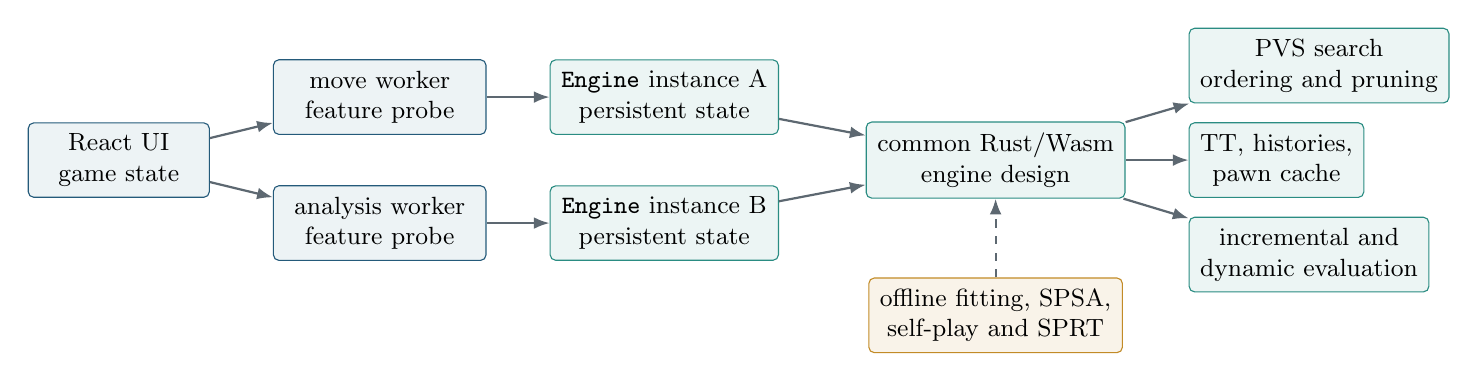
\begin{tikzpicture}[
  font=\small,
  node distance=6mm and 8mm,
  box/.style={draw=mojoblue, rounded corners=2pt, fill=mojolight,
              minimum height=8mm, align=center, inner sep=4pt},
  core/.style={box, draw=mojoteal, fill=mojoteal!9},
  offline/.style={box, draw=mojogold, fill=mojogold!10},
  arrow/.style={-{Latex[length=2mm]}, thick, draw=mojogray}
]
  \node[box, minimum width=23mm] (ui) {React UI\\game state};
  \node[box, right=of ui, yshift=8mm, minimum width=27mm] (move) {move worker\\feature probe};
  \node[box, right=of ui, yshift=-8mm, minimum width=27mm] (analysis) {analysis worker\\feature probe};
  \node[core, right=of move, minimum width=29mm] (engine1) {\code{Engine} instance A\\persistent state};
  \node[core, right=of analysis, minimum width=29mm] (engine2) {\code{Engine} instance B\\persistent state};
  \node[core, right=11mm of engine1, yshift=-8mm, minimum width=29mm] (engine) {common Rust/Wasm\\engine design};
  \node[core, right=of engine, yshift=12mm] (search) {PVS search\\ordering and pruning};
  \node[core, right=of engine] (state) {TT, histories,\\pawn cache};
  \node[core, right=of engine, yshift=-12mm] (eval) {incremental and\\dynamic evaluation};
  \node[offline, below=10mm of engine] (tools) {offline fitting, SPSA,\\self-play and SPRT};

  \draw[arrow] (ui) -- (move);
  \draw[arrow] (ui) -- (analysis);
  \draw[arrow] (move) -- (engine1);
  \draw[arrow] (analysis) -- (engine2);
  \draw[arrow] (engine1) -- (engine);
  \draw[arrow] (engine2) -- (engine);
  \draw[arrow] (engine) -- (search);
  \draw[arrow] (engine) -- (state);
  \draw[arrow] (engine) -- (eval);
  \draw[arrow, dashed] (tools) -- (engine);
\end{tikzpicture}}
\caption{\engine{} execution architecture.  The move and analysis workers own
separate engine instances; the common-design box denotes shared implementation,
not shared runtime state.  The dashed arrow is an offline configuration path.}
\label{fig:architecture}
\end{figure*}

\Cref{fig:architecture} separates the interactive and offline paths.  The
Wasm-facing \code{Engine} accepts FEN plus prior positions, exposes one
completed depth at a time, and returns plain principal-variation data.  A
persistent \code{SearchCore} keeps its transposition table and learned
ordering histories across iterative depths and adjacent positions.  The only
board mutation occurs in immutable child positions supplied by safe Rust APIs;
crate-wide \code{unsafe\_code} is forbidden.

The browser owns two workers.  The \emph{move} instance performs the
time-critical search that chooses a move.  The \emph{analysis} instance may
compute MultiPV output continuously.  A Wasm call is synchronous within its
worker; therefore, placing both workloads behind one instance would allow a
queued analysis call to consume a move's nominal budget before the move search
started.  Isolation makes the budget a property of the move computation rather
than of queueing order.

At startup, each worker validates a small SIMD module and chooses either the
baseline or \code{+simd128} artifact.  WebAssembly supplies compact,
validated, language-independent code and predictable interoperability with a
host environment \citep{haas2017wasm}.  Cross-origin-isolated deployments add
a \code{SharedArrayBuffer} stop word.  The Rust search polls it with atomic
loads between adaptively sized node batches; environments without shared
memory fall back to cancellation between completed depths.  The design remains
functional in both cases, but prompt mid-iteration cancellation requires the
appropriate COOP/COEP headers.

\section{Search Design}

\begin{figure}[t]
\centering
\resizebox{\columnwidth}{!}{%
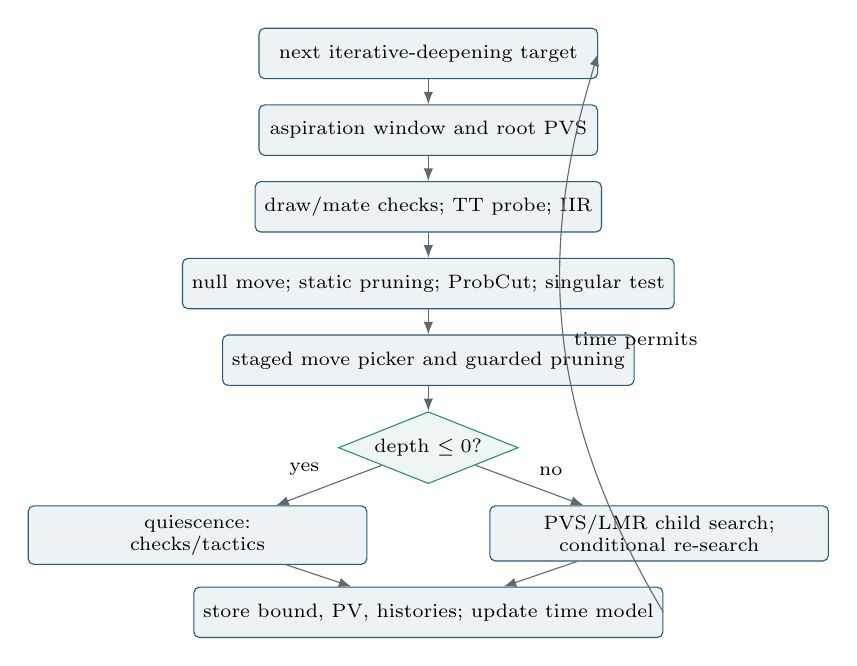
\begin{tikzpicture}[
  font=\scriptsize,
  node distance=3.2mm,
  stage/.style={draw=mojoblue, rounded corners=2pt, fill=mojolight,
                minimum width=43mm, minimum height=6.4mm, align=center},
  decision/.style={diamond, draw=mojoteal, fill=mojoteal!8,
                   aspect=2.5, align=center, inner sep=1.5pt},
  arrow/.style={-{Latex[length=1.6mm]}, draw=mojogray}
]
  \node[stage] (id) {next iterative-deepening target};
  \node[stage, below=of id] (asp) {aspiration window and root PVS};
  \node[stage, below=of asp] (tt) {draw/mate checks; TT probe; IIR};
  \node[stage, below=of tt] (sel) {null move; static pruning; ProbCut; singular test};
  \node[stage, below=of sel] (pick) {staged move picker and guarded pruning};
  \node[decision, below=of pick] (depth) {depth $\leq 0$?};
  \node[stage, below left=5mm and 2mm of depth] (q) {quiescence:\\checks/tactics};
  \node[stage, below right=5mm and 2mm of depth] (child) {PVS/LMR child search;\\conditional re-search};
  \node[stage, below=13mm of depth] (store) {store bound, PV, histories; update time model};
  \draw[arrow] (id) -- (asp);
  \draw[arrow] (asp) -- (tt);
  \draw[arrow] (tt) -- (sel);
  \draw[arrow] (sel) -- (pick);
  \draw[arrow] (pick) -- (depth);
  \draw[arrow] (depth) -- node[above left]{yes} (q);
  \draw[arrow] (depth) -- node[above right]{no} (child);
  \draw[arrow] (q) -- (store);
  \draw[arrow] (child) -- (store);
  \draw[arrow, bend left=24] (store.east) to node[right]{time permits} (id.east);
\end{tikzpicture}}
\caption{Search control flow.  The ordering is significant: cheap bound and
static tests precede move construction, while reduced searches are verified
when they can change alpha.}
\label{fig:search-flow}
\end{figure}

\subsection{Iterative deepening and root search}

The public analysis operation searches exactly one requested depth, while the
worker drives iterative deepening.  This division gives JavaScript a safe
cancellation and reporting boundary without duplicating search logic.  Within
one depth, the previous iteration's score centers a 20-centipawn aspiration
window.  A fail-low or fail-high widens only the failed side; after four
retries, the search falls back to the full interval.  Mate-range scores bypass
aspiration because their distance-sensitive representation should not be
clipped around an ordinary centipawn estimate.

At the root, the first move receives a full-window search.  Later moves first
receive a zero-window PVS probe and are re-searched only when the probe lies
between alpha and beta.  Root order persists the previous score and subtree
node count for each move, placing a previously strong and expensive move
early.  MultiPV repeats the root search while excluding already selected root
moves.  Excluded searches do not overwrite the primary root transposition
entry, preventing a second-best line from displacing the principal move in the
next iteration.

The worker stops deepening using more than elapsed wall time.  It tracks score
stability, how much work concentrated in the best root move, and a smoothed
effective branching factor (EBF).  The last iteration time and EBF predict the
next iteration's cost.  A stable, inexpensive decision can stop near half the
nominal budget; a score drop or unstable best move allows up to roughly 80\%.
The EBF gate blocks an iteration predicted not to fit, except when the soft
fraction indicates that extra effort is warranted.  These policies explain
why a larger limit need not increase completed depth in every row of
\Cref{fig:timed-depth}: the engine may begin and time out in a deeper
iteration while still returning the last complete result.

\subsection{Transpositions, draws, and terminal scores}

The transposition table contains $2^{18}$ cache-line-aligned buckets, each
holding four 16-byte entries, for $2^{20}$ entries and 16 MiB total.  An entry
stores a 64-bit key, encoded move, score, optional static evaluation, signed
depth, bound type, and six-bit generation.  Exact, lower, and upper bounds are
consumed only when their stored depth is sufficient.  Mate scores are adjusted
by ply on store and load so that transposing into a line preserves preference
for a shorter mate or longer defense.  Same-key shallow writes do not replace
deeper results; collision replacement balances depth and age.

Search keys incorporate both position repetition state and the halfmove clock.
The latter is necessary because a visually identical board near the fifty-move
boundary has different legal value.  The search detects the fifty-move rule,
insufficient material, and threefold repetition from real prior positions and
the current path.  Null moves are marked by a path boundary and cannot create a
fictional repetition against real game history.  Checkmate scores are
$\pm(30000-p)$ at ply $p$; stalemate and detected rule draws score zero.

\subsection{Ordering and selective search}

The staged move picker delays work until it can matter.  It returns a legal TT
move first, generates tactical moves ordered by victim value and capture
history, and runs static exchange evaluation (SEE) only as each tactical move
is selected.  Non-losing tactics precede killers, the countermove, and a threat
move learned from a failed null search.  Quiet moves then use main history plus
one- and two-ply continuation history; losing captures are deferred to the
end.  A root-specific picker uses earlier iteration scores and subtree effort.

\begin{table*}[t]
\centering
\small
\caption{Selective mechanisms in \engine{}.  The safeguards are part of the
algorithm: they constrain where a heuristic assumption may discard or reduce
work.}
\label{tab:selectivity}
\begin{tabularx}{\textwidth}{@{}p{0.16\textwidth}p{0.34\textwidth}X@{}}
\toprule
Mechanism & Action & Principal safeguards \\
\midrule
Null move & Reduced null-window search with depth-dependent reduction; record a threat after fail-low & Non-PV, not in check, non-pawn material, depth $\geq3$, halfmove clock $<90$; verification at depth $\geq10$ \\
Reverse futility / razoring & Static fail-high cutoff or shallow fail-low quiescence probe & Non-PV, not in check, non-mate window; bounded to shallow depths and checked for legal moves \\
ProbCut & Search promising captures at depth $d-4$ against $\beta+180$ & Depth $\geq5$, non-PV, not in check, SEE-good captures only; store a reduced-depth lower bound \\
Late-move reduction & Reduce late quiet zero-window probes according to depth and move index & No reduction for captures or evasions; adjust for PV/cut node, checks, history, improving eval; re-search on alpha improvement \\
Move pruning & SEE, late-move, history, and futility rejection & Non-PV, not in check, not first move, not checking, not a detected threat defense; shallow-depth bounds \\
Singular extension & Exclusion search extends a uniquely strong TT move by one or two plies & Depth $\geq7$, sufficiently deep lower/exact TT entry, non-mate score, global two-extension budget \\
Qsearch delta & Skip an exchange that cannot reach alpha even with captured material plus margin & Never while in check; retain promotions and checks; reject SEE-losing captures first \\
\bottomrule
\end{tabularx}
\end{table*}

Late-move reductions are precomputed in a 32-by-64 table with approximately
logarithmic growth in depth and move index.  Context then modifies the base
reduction: PV nodes, checking moves, improving evaluations, and strong history
reduce it; cut nodes and poor history increase it.  Any reduced probe that
raises alpha is repeated at full depth, followed by a full-window re-search if
it remains inside the window.  Thus LMR is a speculative allocation of depth,
not an unconditional acceptance of a reduced score.

Null-move pruning uses reduction $R=2+\lfloor d/4\rfloor$.  At depth ten and
above, a null fail-high triggers a verification search from the original
position with null pruning disabled.  The engine also recovers the null line's
threat move after fail-low and promotes defenses against that threat in
ordering and pruning.  The material and halfmove guards specifically address
the zugzwang and rule-boundary failure modes described in the null-move
literature \citep{donninger1993null}.

ProbCut and singular extension make opposite predictions from deeper TT or
reduced-search evidence.  ProbCut asks whether a good capture already exceeds
a raised beta at reduced depth.  Singular extension performs an exclusion
search without the TT move; a large fail-low marks that move as unique, while
multiple viable alternatives can produce a multi-cut or a negative extension.
Check extensions and singular extensions share a two-ply per-line budget,
preventing unbounded growth.

At depth zero, fail-soft quiescence searches all legal evasions while in check,
or captures and promotions otherwise.  It retains a stand-pat lower bound only
when standing pat is legal.  SEE and delta pruning remove losing or
insufficient captures, except promotions and moves giving check.  Quiescence
results are stored as depth-zero TT bounds and can be reused by later probes.

\section{Evaluation and Learning}

\subsection{Tapered handcrafted evaluation}

The evaluator returns a side-to-move-relative score compatible with
\cref{eq:negamax}.  Material and piece-square values are packed as signed
midgame and endgame 16-bit halves of one 32-bit integer.  Additions therefore
update both components together.  With phase $\phi\in[0,24]$, the white-frame
score is
\begin{equation}
 E_{\mathrm{white}}=
 \frac{\phi E_{\mathrm{MG}}+(24-\phi)E_{\mathrm{EG}}}{24}.
 \label{eq:taper}
\end{equation}
Minor pieces contribute one phase unit, rooks two, queens four, and pawns and
kings zero.  The result is converted to the side-to-move frame, receives a
tempo bonus, and is finally scaled for draw proximity.

An \code{EvalAccumulator} travels with every searched position.  Moving a
piece subtracts its material and piece-square contribution at the origin and
adds the destination contribution; captures, en passant, promotion, and
castling have explicit updates.  The same accumulator maintains phase and a
pawn-only hash.  Debug builds compare incremental children against full
recomputation across move types.

Terms that depend only on pawn placement are stored in a direct-mapped 128-KiB
pawn cache.  The cached record contains packed structure score and passed-pawn
bitboards.  Doubled, isolated, connected, backward, passed, and protected
passed pawns are computed here.  King-distance bonuses for passers are
deliberately excluded because two boards with the same pawn key can have
different king locations.

Dynamic scanning walks knights, bishops, rooks, queens, and kings once.  It
accumulates safe mobility, attack maps, attacks into each king zone, and threat
classes.  A nonlinear 32-entry king-danger curve combines the number and type
of attackers, attacked king-zone squares, safe checks, pawn shelter, and pawn
storms.  Additional terms cover the bishop pair, open and semi-open rook
files, rooks behind passers or on the seventh rank, minor-piece outposts,
hanging pieces, and attacks by pawns or minors on more valuable pieces.
Opposite-colored-bishop endings scale the complete score toward zero.

Bare-king endings need a gradient before mate appears in the horizon.  The
endgame component rewards driving the defending king toward an edge, bringing
the attacking king closer, and confining it with a rook.  Bishop-and-knight
mate instead rewards the corner controlled by the bishop.  Exact KPK positions
override this guidance.  At initialization, a monotone fixed-point procedure
classifies $2\cdot24\cdot64\cdot64$ normalized states and packs the winning set
into 24 KiB.  File and color symmetry map every legal KPK board into that
domain; wins receive a large signed score and known draws return zero.  This is
a small compute-at-initialization instance of retrograde analysis
\citep{thompson1986retrograde}.

The fifty-move rule is integrated twice.  Search returns an exact draw at 100
half-moves, while evaluation before that boundary is damped toward zero.  This
prevents a large heuristic score at half-move 99 from obscuring the immediate
rule constraint.  The same rule-aware key prevents unsafe TT reuse across
different halfmove clocks.

\subsection{Correction history}

The raw evaluator has repeatable residual error.  Three side-indexed correction
tables learn bounded adjustments keyed by pawn structure, material counts, and
non-pawn piece placement.  Together they occupy 192 KiB.  At a quiet searched
node, an exact or compatible bound trains the residual between corrected
static evaluation and search result; capture fail-highs are excluded because
their tactical score is a poor training target.  A depth-dependent weighted
update saturates each entry, and the three table values contribute a bounded
centipawn correction.  This is online calibration of the existing evaluator,
not a replacement value function.

\subsection{Offline parameter fitting}

The evaluator exposes 887 tunable parameters: piece-square cells and paired
midgame/endgame weights for material, pawn structure, mobility, king attack,
passers, threats, outposts, and rook features.  A training row contains a game
result $y\in\{0,\tfrac12,1\}$ and FEN.  The tuner removes non-quiet positions,
deduplicates board hashes, averages conflicting labels, and deterministically
partitions examples into training and validation sets.  Labels are transformed
into the side-to-move frame used by the evaluator.

For feature vector $x$ and weight vector $w$, the predicted result is
\begin{equation}
 p(y=1\mid x)=\sigma\!\left(\frac{x^\top w}{K}\right),\qquad K=400,
 \label{eq:logistic}
\end{equation}
and gradient descent minimizes cross-entropy plus a small $L_2$ penalty toward
the checked-in weights.  Material anchors prevent the fit from changing the
scale arbitrarily, and left--right piece-square symmetry is restored before
emission.  This implements outcome-labeled logistic feature fitting in the
tradition of \citet{buro1995features}; the repository names the workflow
``Texel tuning.''  Generated source contains only deltas from readable
hand-authored bases.

Six search constants---aspiration width, reverse-futility margin, two futility
margins, ProbCut margin, and quiescence delta margin---form a separate SPSA
surface.  In iteration $k$, random signs $\Delta_k$ define bounded candidates
$\theta_k^{\pm}=\theta_k\pm c_k\Delta_k$.  A color-swapped self-play match
supplies a noisy score difference, and the update follows the simultaneous
perturbation estimate \citep{spall1992spsa}.  Seeds, bounds, schedules, opening
count, and time control are recorded.  Tuning output remains exploratory until
a 128-opening, 100-ms-per-move SPRT accepts the $+10$ Elo hypothesis with
$\alpha=\beta=0.05$.  The acceptance policy follows Wald's sequential testing
framework \citep{wald1945sprt}; it does not turn a small tuning match into a
strength claim.

\section{Experimental Method}

All measurements use repository revision \code{aeb6b5b}.  The host is an Intel
Core Ultra 5 235 with 14 visible cores and 24 MiB L3 cache, running 64-bit Linux
under WSL2.  Node.js 24.18.0 executes the Wasm modules; the artifacts were
produced with Rust 1.96.1 and wasm-pack 0.15.0.  Although the host has multiple
cores, each engine search is single-threaded.  Results therefore describe this
Node/V8 environment and must not be generalized to all browsers or machines.

The bundled benchmark defines four FENs: the initial position, a tactical
position with castling rights and contact in the center, a representative
middlegame, and a rook-and-pawn endgame.  Each sample creates a fresh engine so
that an earlier position or MultiPV configuration cannot warm the TT.  The
stop-flag path matches a cross-origin-isolated browser.

For throughput, both baseline and \code{+simd128} artifacts search iterative
depths one through nine.  Each position is warmed twice and measured seven
times.  The harness alternates artifact order by repetition to reduce drift.
Node counts, best moves, and final scores must be deterministic; the reported
rate is cumulative nodes divided by the median wall time.  The graph uses
single-PV rows.  MultiPV=3 is retained as a cost check.

For budget behavior, the baseline artifact searches at nominal limits of 100,
500, and 1000 ms.  Three independent repetitions are summarized by median
wall time and completed depth.  The worker may stop before the limit when its
soft-time and EBF tests predict that the next iteration will not fit.  It may
also spend the limit on an incomplete next depth while reporting the previous
complete result.  Accordingly, the experiment measures achieved depth, not an
assumption that every sample consumes exactly its nominal budget.

Binary measurements use the exact module bytes, gzip, and Brotli quality 11.
Initial and peak linear memory are read from the instantiated Wasm memory.  The
Rust test suite is executed separately in an unoptimized native test profile.
The CSV files used by the plots are shipped with the paper, and the PDF is
generated directly from them using PGFPlots.

\section{Results}

\begin{figure}[t]
\centering
\begin{tikzpicture}
\begin{axis}[
  width=\columnwidth,
  height=0.72\columnwidth,
  ybar,
  bar width=6pt,
  ymin=0,
  ymax=4.4,
  ylabel={Median nodes/s (millions)},
  symbolic x coords={Start,Tactical,Middlegame,Endgame},
  xtick=data,
  x tick label style={rotate=24,anchor=east,font=\scriptsize},
  y tick label style={font=\scriptsize},
  label style={font=\scriptsize},
  legend style={font=\scriptsize,at={(0.5,1.02)},anchor=south,legend columns=2,draw=none},
  grid=major,
  grid style={draw=gray!18},
  enlarge x limits=0.13
]
\addplot+[fill=mojoblue!75,draw=mojoblue]
  table[x=position,y expr=\thisrow{baseline_nps}/1000000,col sep=comma]
  {data/fixed-depth.csv};
\addplot+[fill=mojoteal!70,draw=mojoteal]
  table[x=position,y expr=\thisrow{simd_nps}/1000000,col sep=comma]
  {data/fixed-depth.csv};
\legend{Baseline,SIMD}
\end{axis}
\end{tikzpicture}
\caption{Fixed-depth-9 single-PV throughput.  Bars use seven samples after two
warmups.  Equal node counts make each pair a direct timing comparison.}
\label{fig:throughput}
\end{figure}

\Cref{fig:throughput} shows substantial position dependence.  Baseline median
throughput ranges from 2.17 million nodes/s in the tactical position to 3.67
million in the endgame.  The likely cause is work per node: sliding attacks,
move count, pruning eligibility, and cache reuse differ across positions.
Nodes/s is therefore a property of a workload, not a machine constant.

SIMD produces small, mixed changes: $-0.79\%$ at the start, $+0.49\%$ in the
tactical position, $-1.95\%$ in the middlegame, and $+3.35\%$ in the endgame.
The geometric mean over the four single-PV rows is $+0.26\%$.  Every pair has
identical cumulative nodes, best move, and score, isolating code-generation
speed rather than search divergence.  On this platform the evidence supports
shipping a feature-gated variant at low size cost, but not describing SIMD as
uniformly faster.

MultiPV illustrates a different cost dimension.  At depth nine, baseline
cumulative nodes rise from 44,335 to 122,770 at the start, 66,098 to 272,613 in
the tactical position, 111,328 to 306,474 in the middlegame, and 29,990 to
92,973 in the endgame.  Three lines cost between 2.77 and 4.12 times the
single-PV work in this small suite.  Isolating background analysis in its own
worker is consequently important even when one search is individually fast.

\begin{figure}[t]
\centering
\begin{tikzpicture}
\begin{axis}[
  width=\columnwidth,
  height=0.72\columnwidth,
  xlabel={Nominal move budget (ms)},
  ylabel={Completed depth (plies)},
  xmin=70,xmax=1030,
  ymin=8,ymax=22,
  xtick={100,500,1000},
  ytick={10,12,14,16,18,20,22},
  tick label style={font=\scriptsize},
  label style={font=\scriptsize},
  legend style={font=\tiny,at={(0.5,1.02)},anchor=south,legend columns=2,draw=none},
  grid=major,
  grid style={draw=gray!18}
]
\addplot+[mark=*,thick,color=mojoblue]
  table[x=budget_ms,y=start,col sep=comma]{data/timed-depth.csv};
\addplot+[mark=square*,thick,color=mojoteal]
  table[x=budget_ms,y=tactical,col sep=comma]{data/timed-depth.csv};
\addplot+[mark=triangle*,thick,color=mojogold]
  table[x=budget_ms,y=middlegame,col sep=comma]{data/timed-depth.csv};
\addplot+[mark=diamond*,thick,color=mojogray]
  table[x=budget_ms,y=endgame,col sep=comma]{data/timed-depth.csv};
\legend{Start,Tactical,Middlegame,Endgame}
\end{axis}
\end{tikzpicture}
\caption{Completed single-PV depth under nominal move budgets.  Values are
medians of three fresh-engine samples; early stopping and timed-out next
iterations are part of the measured policy.}
\label{fig:timed-depth}
\end{figure}

\Cref{fig:timed-depth} reflects both branching and time management.  The
endgame reaches depth 13 at 100 ms and depth 21 at 1000 ms, while the other
positions reach depths 10--11 and 14, respectively.  The start and tactical
rows report depth 14 at both 500 and 1000 ms.  In those samples the larger
budget was spent attempting a deeper iteration that did not complete; the
last fully searched line remained depth 14.  This behavior is intentional:
publishing a partial tree as a completed depth would make depth and score
misleading.  The engine can return a sound partially searched root line for a
timed-out single-PV iteration, but labels it separately and does not substitute
it for the completed-depth benchmark field.

\begin{table}[t]
\centering
\small
\caption{Wasm artifact and memory measurements.  MiB values use $2^{20}$
bytes.}
\label{tab:artifacts}
\begin{tabular}{@{}lrr@{}}
\toprule
Metric & Baseline & SIMD \\
\midrule
Raw module (bytes) & 1,456,876 & 1,459,636 \\
gzip (bytes) & 223,268 & 223,553 \\
Brotli-11 (bytes) & 132,934 & 133,266 \\
Initial memory (MiB) & 2.56 & 2.56 \\
Peak memory (MiB) & 19.69 & 19.69 \\
\bottomrule
\end{tabular}
\end{table}

Both gzip sizes in \Cref{tab:artifacts} are below the 250,000-byte ceiling.
The SIMD module adds 2,760 raw bytes but only 285 gzip bytes.  Peak linear
memory is dominated by the 16-MiB TT plus ordering, correction, pawn-cache,
board, and Wasm runtime storage.  Important fixed structures include a 288-KiB
continuation-history table, a 192-KiB correction history, a 128-KiB pawn cache,
a 24-KiB KPK bitbase, a 9-KiB capture history, and a 2-KiB LMR table.  These
sizes are asserted in tests where layout is part of the design.

The native Rust suite passes 75 tests.  Coverage includes standard perft
positions, legal PVs, forced mate, repetition and fifty-move draws, incremental
evaluation agreement, KPK normalization, SEE thresholds, TT collision and
mate-score behavior, every move-picker stage, pruning guards, timeout
semantics, clock calibration, MultiPV distinctness, and memory footprints.
Tests cannot establish playing strength, but they protect invariants that
selective search could otherwise violate silently.

\section{Discussion and Limitations}

The implementation demonstrates that compactness and sophistication are not
opposites.  Most search features are small control policies over shared data:
the TT move feeds root order, PVS, singular tests, and quiescence; a null search
can yield either a cutoff or an ordering threat; history affects ordering,
pruning, and LMR.  This reuse keeps the binary small, but it also makes
interactions difficult to reason about in isolation.  Guard-focused tests and
fixed-depth determinism are therefore as important as tests of individual
score formulas.

The evaluator makes a similar decomposition by update frequency.  Material,
piece-square score, phase, and pawn key change incrementally with every move.
Pawn relations are cached across boards with the same pawns.  Mobility, king
safety, and tactical threats are recomputed because their occupancy-dependent
attack sets change broadly.  This division avoids both a full evaluator at
every node and a fragile attempt to update every dynamic relation.

The benchmark has several limitations.  Four hand-selected positions do not
represent the distribution of a game, and nodes have unequal cost.  Median
timing on one Node/V8 build does not characterize Chrome, Firefox, Safari,
mobile CPUs, thermal throttling, or native Rust.  The SIMD comparison measures
two compiler artifacts but does not attribute changes to particular Wasm
instructions.  The timed experiment has only three repetitions and reports
completed integer depths, a coarse outcome.  No confidence intervals are
claimed.

Most importantly, throughput is not strength.  A pruning change can search
fewer nodes and play worse; a richer evaluator can search fewer nodes per
second and play better.  This paper reports no absolute Elo because no rated
opponent pool and calibrated time control were evaluated.  The repository's
color-swapped SPRT process is suitable for accepting a candidate relative to a
fixed baseline, not assigning a universal rating.  Likewise, comparing an
artifact with itself can validate determinism and harness symmetry but cannot
support a strength difference.

Future evaluation should use a versioned opening suite, an independent
baseline artifact, enough paired games to reach a predeclared SPRT boundary,
and browser-native measurements across engines and devices.  Search ablations
would quantify each heuristic's node and strength contribution, though such
experiments must retune interacting constants or explicitly acknowledge that
they measure a perturbed configuration.  Hardware performance counters are not
available in ordinary browser execution, so native profiling can complement,
but not replace, deployed Wasm measurements.

\section{Conclusion}

\engine{} integrates established computer-chess techniques into a constrained
browser system.  Its search combines PVS, transposition reuse, staged ordering,
quiescence, and guarded selectivity; its evaluator combines incremental
tapered scores, cached pawn knowledge, dynamic attacks, learned correction,
and an exact KPK exception.  Separate workers and atomic cancellation preserve
interactive time semantics, while dual Wasm artifacts remain under a strict
download limit.  Local measurements show deterministic fixed-depth behavior,
position-dependent throughput, and only a marginal aggregate SIMD difference
on the tested host.  The broader lesson is methodological: report search work,
runtime, size, and strength as distinct quantities, and validate each with an
experiment designed for that quantity.

\bibliographystyle{plainnat}
\bibliography{references}

\end{document}
